\documentclass[11pt]{article}

\usepackage{hyperref}
\usepackage{graphicx}
\usepackage{xcolor}

%opening
\title{Saddle Point Problems or Min-Max Problems}
\date{}
\author{
	Pavlenko, Nikolay\\
	\texttt{n.pavlenko@innopolis.university}
	\and
	Dyussenova, Ashera\\
	\texttt{a.dyussenova@innopolis.university}
}

\begin{document}

\maketitle

\section*{Introduction:}

Saddle point or min-max problems are more difficult problems than minimization problems. Meanwhile, min-max problems often arise in machine learning. The goal of this project is to understand the difference between min-max problems and minimization problems, and to learn methods for min-max problems. \\

This project is built upon an analysis of two papers: \href{https://openreview.net/pdf?id=r1laEnA5Ym}{\textbf{A Variational Inequality Perspective on Generative Adversarial Networks}} and \href{https://proceedings.neurips.cc/paper/2019/file/4625d8e31dad7d1c4c83399a6eb62f0c-Paper.pdf}{\textbf{On the Convergence of Single-Cell Stochastic Extra-Gradient Methods}}.

In order to comply with the requirement to have a single \LaTeX\ file in the root directory of the project, this file will cover detailed analysis of both papers, though they will be contained in separate sections. Analysis of the problem in general and conclusion will follow the rest of the report in the final section of the .tex file.

\section{A Variational Inequality Perspective on Generative Adversarial Networks:}

	\subsection{Problem Statement:}
	
	\subsection{Main Idea of the Approach:}
	
	\subsection{Theory and Background:}
		
		\subsubsection{Related Work:}
		
		\subsubsection{Theoretical Framework:}
		
		\subsubsection{Key Features:}
		
		\subsubsection{Causes behind Good Performance:}
		
		\subsubsection{Improvements over Older Methods:}
	
	\subsection{Essence of Proof:} %I don't like the name, rename if you have any good ideas
	
	\subsection{Experiments and Results:}

\section{On the Convergence of Single-Cell Stochastic Extra-Gradient Methods:}

	\subsection{Problem Statement:}
        Landscape of the loss function in GANs does not resemble the minimization problem, but that of a min-max game which in our words could be called a \textbf{variational inequality}. They have gained significant attention in machine learning, offering a flexible framework beyond ordinary loss function minimization, particularly in generative adversarial networks (GANs) and deep learning systems. The optimal $O(1/t)$ convergence rate for solving smooth monotone variational inequalities is achieved by the Extra-Gradient (EG) algorithm and its variants. These methods require two projections and two oracle calls per iteration, making them costly compared to standard methods like Forward-Backward. Reducing this cost is the main goal of the current paper.
	
	\subsection{Main Idea of the Approach:}
        The primary focus of this research is to investigate and quantify the convergence behavior of single-call stochastic extra-gradient methods when solving variational inequalities. By understanding the underlying mechanisms of these algorithms, the paper aims to provide valuable insights into their applicability and efficiency, especially in the realm of non-monotone variational inequalities.
	
	\subsection{Theory and Background: }
 
        Variational inequalities, encompassing diverse problems like minimization, saddle-points, Nash equilibria, and fixed-point problems, serve as a foundational framework in optimization. The EG algorithm, with its variants, has been pivotal in solving monotone variational inequalities. However, the computational cost involved has led to the exploration of single-call variants, sparking a significant area of research. This paper delves into these single-call methods, studying their properties and convergence rates in both deterministic and stochastic scenarios.
	
		\subsubsection{Related Work: }
  
        Existing research has explored various algorithms, such as Forward-Backward-Forward (FBF) and gradient extrapolation mechanisms like Popov's modified Arrow-Hurwicz algorithm, to reduce the number of oracle calls and projections. Among these, single-call extra-gradient methods, including Past Extra-Gradient (PEG), Reflected Gradient (RG), and Optimistic Gradient (OG), have gained prominence for their efficiency in approximating missing gradients while making a single oracle call per iteration.
		
		\subsubsection{Theoretical Framework: }
  
        In the context of variational inequalities, the Extra-Gradient algorithm involves two projections and oracle calls per iteration. Single-call variants like PEG, RG, and OG perform a single oracle call while approximating missing gradients differently. These algorithms converge at the optimal O(1/t) rate under certain assumptions.
		
		\subsubsection{Key Features: }
        \begin{itemize}
            \item Variational inequalities provide a flexible framework in machine learning beyond traditional loss function minimization.
            \item Extra-Gradient and its variants achieve optimal O(1/t) convergence rates.
            \item Single-call extra-gradient methods, such as PEG, RG, and OG, approximate missing gradients with a single oracle call per iteration.
        \end{itemize}
		
		\subsubsection{Causes behind Good Performance: }
  
        The performance of single-call extra-gradient methods is attributed to their ability to anticipate the landscape of the problem by approximating missing gradients while making only one oracle call per iteration. These methods achieve optimal convergence rates in both deterministic and stochastic variational inequalities under suitable conditions.
		
		\subsubsection{Improvements over Older Methods: }
  
        Single-call extra-gradient methods significantly reduce the computational cost associated with multiple oracle calls and projections. They retain the anticipatory properties of the original Extra-Gradient algorithm while making efficient use of oracle resources.
	
	\subsection{Essence of Proof: }
        
        The proofs for the convergence rates of single-call extra-gradient methods involve intricate analyses. Techniques such as quasi-descent inequalities and probabilistic arguments are employed to establish convergence properties. For stochastic variational inequalities, careful consideration of noise realizations and conditional bias is necessary to prove convergence rates.
 %I don't like the name, rename if you have any good ideas
	
	\subsection{Experiments and Results:}
 
        Experimental results demonstrate the efficiency of single-call extra-gradient methods in both deterministic and stochastic variational inequalities. These methods consistently outperform the traditional Extra-Gradient algorithm in terms of convergence speed, especially in scenarios where computational resources are limited.
        \begin{figure}[h]
            \centering
            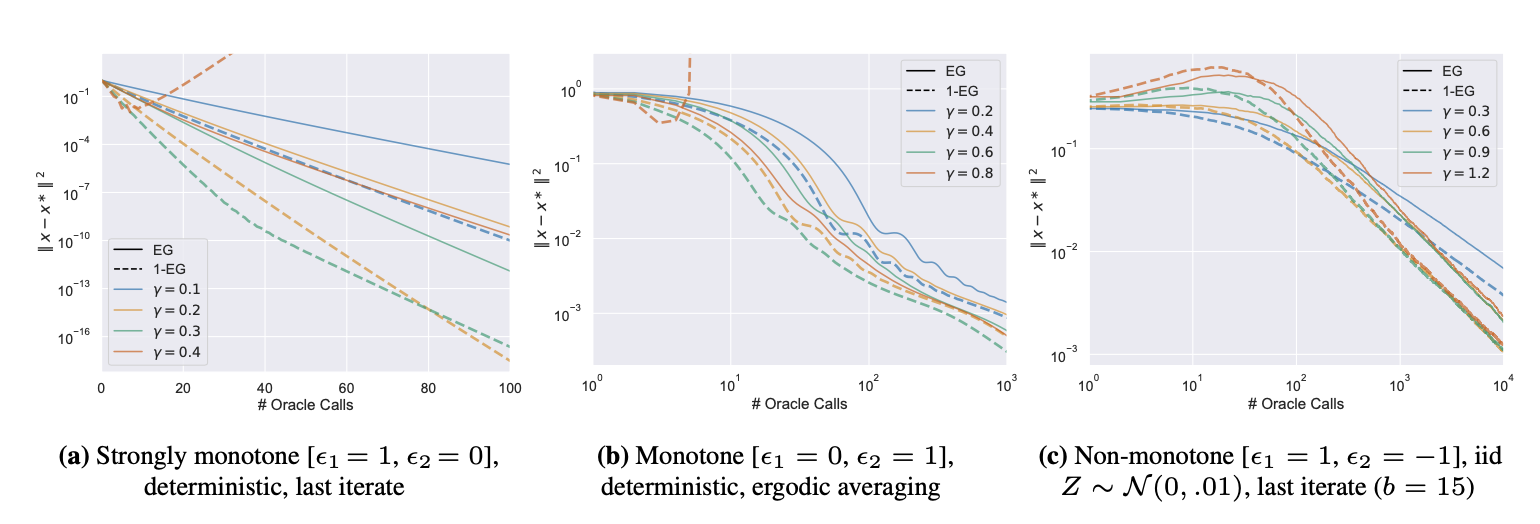
\includegraphics[scale=0.5]{pictures/pic1.png}
            \caption{Illustration of the performance of EG and 1-EG in the (a priori non-monotone) saddle-point problem $\mathcal{L}(\theta, \phi) = 2 \epsilon_1 \theta^T A_1 \theta + \epsilon_2 (\theta^T A_2 \theta)^2 - 2 \theta_1 \phi^T B_1 \phi - \epsilon_2 (\phi^T B_2 \phi)^2 + 4\theta^T C \phi$ }
            \label{fig:label}
        \end{figure}
 
	
\section{Conclusion:}

\end{document}